
\begin{figure}[htp]
  \centering
\begin{minipage}{.46\textwidth}
  \centering
  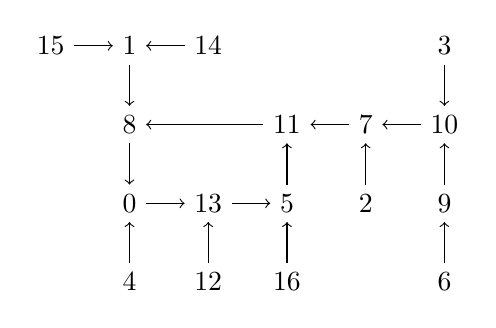
\begin{tikzpicture}
    \node at (2,1) (0) {0};
    \node at (2,3) (1) {1};
    \node at (5,1) (2) {2};
    \node at (6,3) (3) {3};
    \node at (2,0) (4) {4};
    \node at (4,1) (5) {5};
    \node at (6,0) (6) {6};
    \node at (5,2) (7) {7};
    \node at (2,2) (8) {8};
    \node at (6,1) (9) {9};
    \node at (6,2) (10) {10};
    \node at (4,2) (11) {11};
    \node at (3,0) (12) {12};
    \node at (3,1) (13) {13};
    \node at (3,3) (14) {14};
    \node at (1,3) (15) {15};
    \node at (4,0) (16) {16};
    \draw[->] (0) -- (13);
    \draw[->] (1) -- (8);
    \draw[->] (2) -- (7);
    \draw[->] (3) -- (10);
    \draw[->] (4) -- (0);
    \draw[->] (5) -- (11);
    \draw[->] (6) -- (9);
    \draw[->] (7) -- (11);
    \draw[->] (8) -- (0);
    \draw[->] (9) -- (10);
    \draw[->] (10) -- (7);
    \draw[->] (11) -- (8);
    \draw[->] (12) -- (13);
    \draw[->] (13) -- (5);
    \draw[->] (14) -- (1);
    \draw[->] (15) -- (1);
    \draw[->] (16) -- (5);
  \end{tikzpicture}
  \caption{Gráfico del polinomio en el campo finito $\Z_{17}$.}
\end{minipage}
\end{figure}
